\documentclass{article}

\usepackage{listings}
\usepackage{graphicx}

\begin{document}

\begin{abstract}
This article is created within the CAS program Maxima.
and shows (1) algebraic differentiation (2) plotting, and (3) listings,
which are believed to be the most commonly used aspects of an article.
\end{abstract}

\section{Introduction}

Writing scientific articles is commonly done with \LaTeX.
Algebraic manipulations can be done by a CAS, for example Maxima, Maple or Mathematica.
Of these examples, Maxima is the only free and open-source program.
Would it be possible to write a \LaTeX article within Maxima?
If yes, would it be elegant enough?

\section{Materials and methods}

A script executes the process from Maxima file to \LaTeX-formatted document in two steps.
The first step executes the Maxima script to create a \LaTeX (.tex) file.
The second step converts the \LaTeX file to Portable Document Format (.pdf).
The script does not require user intervention.

The Maxima script consists out of two parts:
algebraic manipulations and \LaTeX output

The algebraic manipulations demonstrated are: 
(1) defining a function
(2) calculate its derivative and,
(3) plot this derivative.

The second part uses these algebraic results to create a \LaTeX (.tex) file.
It creates an article displaying the formula's, the single plot in
the Results section.
In the Appendix, it shows: 
(1) the bash script to create a PDF from the Maxima script
(2) the Maxima script
(3) the generated \LaTeX code

\section{Results}

This is the formula for f:

$$f\left(x\right)=x^3+2\,x^2+3\,x+4$$

This is the formula for g, the derivative of f to x:

$$g\left(x\right)=3\,x^2+4\,x+3$$

Which looks plotted as such:

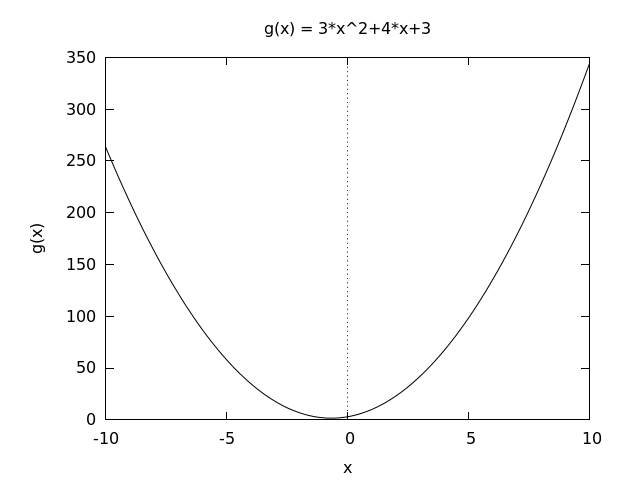
\includegraphics[scale=0.5]{/home/richel/GitHubs/Maxima/create_tex_article_simple_output.png}

\appendix

\section{Script file}

\lstinputlisting[language=C++,showstringspaces=false,breaklines=true,frame=single]{create_tex_article_simple.sh}

\section{Maxima file}

\lstinputlisting[language=C++,showstringspaces=false,breaklines=true,frame=single]{create_tex_article_simple.txt}

\section{\LaTeX file}

\lstinputlisting[language=tex,showstringspaces=false,breaklines=true,frame=single]{create_tex_article_simple_output.tex}

\end{document}
